% This is samplepaper.tex, a sample chapter demonstrating the
% LLNCS macro package for Springer Computer Science proceedings;
% Version 2.25 of 2026/09/03
%
\documentclass[runningheads]{llncs}
%
\usepackage[T1]{fontenc}
% T1 fonts will be used to generate the final print and online PDFs,
% so please use T1 fonts in your manuscript whenever possible.
% Other font encondings may result in incorrect characters.
%
\usepackage{float}
\usepackage{newtxtext}       % 
\usepackage[varvw]{newtxmath}       % selects Times Roman as basic font

\usepackage{subcaption}
\usepackage{graphicx}
% Used for displaying a sample figure. If possible, figure files should
% be included in EPS format.
%
% If you use the hyperref package, please uncomment the following two lines
% to display URLs in blue roman font according to Springer's eBook style:
\usepackage[hidelinks]{hyperref}
\usepackage{color}
\renewcommand\UrlFont{\color{blue}\rmfamily}
%\urlstyle{rm}
%

%\setlength{\parindent}{0pt}  % sin sangría
%\setlength{\parskip}{6pt plus 1pt minus 1pt}   % espacio al final de cada párrafo
\setlength{\textfloatsep}{8pt}
\raggedbottom   % evita huecos raros al estirar el espacio

\begin{document}

%
\title{Meta-Research on LLM-assisted peer review: Evaluating agreement and strictness in CLAIM audits}
%
\titlerunning{LLM-Assisted Peer Review in CLAIM Audits}
% If the paper title is too long for the running head, you can set
% an abbreviated paper title here
%
\author{Anonymous} %Alicia Ramos\and Andrea Sánchez\and Mireia Brichs\and Yolanda Romero
%
%\authorrunning{A. Ramos et al.}
% First names are abbreviated in the running head.
% If there are more than two authors, 'et al.' is used.
%
\institute{Universitat Pompeu Fabra\\
%\email{\{aliciamaria.ramos01, mireia.brichs01\}@estudiant.upf.edu}
}
%
\maketitle              % typeset the header of the contribution
%
\begin{abstract}
This study aims to determine how closely three large language models (LLMs), ChatGPT, Claude and Gemini, agree with human assessors when evaluating reporting quality with the Checklist for Artificial Intelligence in Medical Imaging (CLAIM), and whether they are stricter or more lenient. 

The structured, predefined criteria of CLAIM are proposed to make checklist verification a suitable task for the 'LLM-as-a-Judge' paradigm, with the potential to make peer review faster and more consistent.  Previous studies report inconsistent agreement between LLMs and reviewers in unstructured manuscript evaluation, and model-dependent agreement for other reporting guidelines, but none has compared several LLMs with human assessors on CLAIM. We compared the CLAIM 2020 compliance scores of 60 papers, taken from a published systematic review, with those generated by the three LLMs using a single zero-shot prompt and default settings, analysing agreement with Mean Absolute Error (MAE), strictness with Mean Error (ME), differences between models and rank correlation with Holm-corrected tests. 

In general, LLMs were significantly stricter than humans, although Claude and Gemini were more lenient in the performance domain. No LLM ranked papers like human assessors, and no model was best across all domains. To our knowledge, this is the first multi-model comparison on CLAIM; it shows that LLMs should not replace human audits but could serve as supervised screening tools, and it points to prompt calibration, few-shot examples and item-level analyses as next steps. 
\keywords{Peer Review\and Large Language Models \and CLAIM \and  Reporting Quality \and Medical Imaging}
\end{abstract}


\section{Introduction}
Peer review is essential to scientific publishing as it evaluates the quality, reliability and reproducibility of research before publication. However, this process can be time-consuming and subject to variability and subjectivity between reviewers. Large language models (LLMs), such as Claude, ChatGPT and Gemini, could support this process by assisting with specific aspects of manuscript evaluation \cite{ebadi-2025}, but it remains unclear how reliable their assessments are compared with those of human reviewers \cite{suleiman-2024}.

Rather than asking whether LLMs could replace the entire peer review process, this study focuses on a narrower task: assessing the reporting quality of scientific papers with a standardized checklist, the  Checklist for Artificial Intelligence in Medical Imaging (CLAIM). Therefore, the main research question of this study is \textit{how closely do LLMs agree with human assessors when assessing the reporting quality of scientific papers with CLAIM?}. Additionally, the study examines whether LLMs tend to be stricter or more lenient than human assessors, whether agreement differs across models and which one is the most promising to support checklist-based evaluation in peer review.


\subsection{Literature review}
In medical imaging, transparency and reproducibility are fundamental for building trust in the clinical application of artificial intelligence (AI). For this reason, CLAIM was developed by experts as a standardized guideline for reporting AI studies in medical imaging. It is a structured checklist that covers the main sections of a scientific manuscript and addresses key aspects of the research process; including study design, data curation, model training and performance evaluation. Each item can be rated as Yes, No or Not Applicable; accommodating different study methodologies \cite{mongan-2020}. Following its revision in 2024, two additional items were incorporated, increasing the total number of checklist items from 42 to 44 \cite{tejani-2024}.

Because of these standardized, objective and verifiable criteria, recent editorial positions argue that checklist verification should become a mandatory audit during peer review \cite{zhong-2025}. However, applying these checklists consistently is challenging, as the process is time-consuming and varies between reviewers. 

In this context, LLMs have emerged as a potential tool for supporting peer review. Models such as ChatGPT, Claude and Gemini stand out in this context due to their capacity to reason over complex biomedical texts \cite{thirunavukarasu-2023}. Since human reviews can vary considerably due to subjectivity, LLMs might offer more objective assessments. However, their performance in unstructured manuscript evaluation has been inconsistent: studies have reported limited agreement between LLMs and human reviewers, including a potential leniency towards manuscripts with methodological flaws \cite{saad-2024},\cite{suleiman-2024}. In contrast, a blinded study found that, when the evaluation was structured AI-generated reviews were non-inferior to human ones \cite{zancanaro-2026}. This suggests that structured and standardized criteria may improve the consistency of LLM-assisted reviews. 

Recent studies suggest that this approach is feasible: models such as GPT-4 and Claude have been used to audit compliance with reporting guidelines such as CONSORT \cite{tsybulnik-2026}, and a study of neuroimaging papers using the COBIDAS guideline showed that AI-human agreement is possible but depends strongly on the LLM used \cite{pluimer-2026}.


\subsection{Rationale and justification}
Checklist-based assessment is central to systematic reviews, editorial screening and peer review, yet it is time-consuming and not required by all journals \cite{kocak-2024},\cite{kocak-2025}. This is particularly relevant in AI-based medical imaging, where incomplete reporting limits reproducibility and clinical translation. LLMs could make checklist audits faster and more scalable, but only if their judgments align with those of human assessors.

Evidence for CLAIM is still lacking. To our knowledge, no study has compared several LLMs with human assessors on CLAIM compliance scores under the same criteria, or examined whether LLMs are systematically stricter or more lenient than humans. By comparing three LLMs with human assessors, this study indicates which models, and in which CLAIM domains, come close enough to human scores to support reviewers and where human verification is still needed. In this way, it contributes to improving the rigor and efficiency of peer review, in line with the goals of meta-research: studying and improving how research itself is evaluated in the era of AI. 

  


\section{Methodology}
To address the research question, CLAIM evaluations generated by three LLMs were compared with those provided by human reviewers. Those were obtained from a previously published systematic review, which included 209 studies of AI cardiac MRI segmentation. Each study was evaluated using the 42 items of the 2020 version of CLAIM and organised into four domains: Study description, Dataset description, Model description and Model performance (Appendix \ref{app:table}) \cite{alabed2022quality}. It provided descriptive characteristics for each paper, together with compliance scores for each domain. Therefore, all comparisons in this study were performed using domain-level and overall scores rather than individual CLAIM items. The human scores were used as the reference standard, although they may also involve some degree of subjectivity, as acknowledged by the original authors \cite{alabed2022quality}. 

For this meta-research, the first 60 papers in the original dataset with available full texts were selected. Full-text access was obtained either through publicly accessible links or through the institutional access provided by Universitat Pompeu Fabra. 

\subsection{LLMs assessments and compliance score calculation}
Three of the most widely used LLMs were included in the study: Gemini 3.8 Flash (Google), GPT-6 (OpenAI) and Claude Sonnet 5.5 (Anthropic). A new independent Google account was created to avoid any influence from previous conversations, saved information or custom instructions. All models were used with their standard reasoning mode, without enabling extended-reasoning options or changing the default settings. 

The evaluations were generated using the same prompt (Appendix \ref{app:prompt}) for all three models and all 60 papers. It instructed each model to act as an experienced peer reviewer with expertise in artificial intelligence and medical imaging and to evaluate the manuscript according to all 42 items of CLAIM 2020. The full description of each item was included in the prompt. 

For every item, the models were required to provide one of three possible answers: Yes, No or Not Applicable. They were instructed to rely exclusively on information explicitly reported in the manuscript, assess each item independently and avoid assuming that unreported procedures had been performed. When relevant information was missing, the answer had to be No rather than Not Applicable. To ensure consistent and easily comparable outputs, the responses were restricted to 43 lines: the paper’s PDF filename followed by one answer for each of the 42 CLAIM items, without additional explanations.

Each PDF was uploaded together with the complete prompt between November 6th and 9th of 2026. Manuscripts were processed within the same conversation until the usage limit was reached. Processing was then paused until the limit was reset. 

The responses obtained from each model were transferred to an Excel spreadsheet, with one row per paper evaluation and one column per CLAIM item. This resulted in an expanded dataset of 60 papers for each LLM (240 observations). Based on these responses, a compliance score (Equation \ref{eq:compliance}) was calculated for each paper, model and CLAIM domain, as well as for the overall checklist. 

\begin{equation}
\text{Compliance Score} = \frac{\text{Yes}}{\text{Yes}+\text{No}} \times 100
\label{eq:compliance}
\end{equation}

\subsection{Evaluation metrics}
All statistical analyses and visualizations were performed in Python (version 3.13.18) using Jupyter Notebooks. The data were processed using the pandas and NumPy libraries, statistical analyses were conducted using SciPy and statsmodels, and figures were generated using Matplotlib and Seaborn.

%All statistical analyses and visualizations were performed in Python (version 3.13.18) using Jupyter Notebooks. The data were processed using the pandas (version 2.2.3) and NumPy (version 2.4.6) libraries, statistical analyses were conducted using SciPy (version 1.16.3) and statsmodels (version 0.15.0), and figures were generated using Matplotlib (version 3.10.0) and Seaborn (version 0.13.2).

Statistical analyses were performed separately for the four CLAIM domain scores and the overall compliance score, resulting in five outcomes. For each paper, model and outcome, the error was defined as the difference between the LLM score and the corresponding human score, expressed in percentage points.

Before conducting the statistical analyses, scores were prepared for comparison. Tied values were assigned average ranks in the Friedman and Spearman analyses, while zero differences were excluded from the Wilcoxon signed-rank tests. An adjusted p-value below 0.05 was considered statistically significant for all tests. 

To measure agreement with the human reviewers, the mean absolute error (MAE) was calculated for each model and outcome. To assess whether the models tended to be stricter or more lenient than the human reviewers, the mean error (ME), calculated as the average of the signed differences, was used. Negative ME values indicate a stricter evaluation and positive values a more lenient one. Whether these differences were statistically significant was tested using a two-sided Wilcoxon signed-rank test on the paired scores. The resulting 15 p-values were adjusted using the Holm method. 

To compare the performance of the three LLMs, the absolute errors relative to the human scores were compared across papers using the Friedman test, separately for each of the five outcomes. Again, the five resulting p-values were adjusted using the Holm method. In addition, pairwise comparisons between the three models were performed for each outcome using two-sided Wilcoxon signed-rank tests on the paired absolute errors, regardless of the Friedman test results. P-values from these pairwise comparisons were adjusted using the Holm method separately for each outcome.

Finally, Spearman’s rank correlation coefficient $(\rho)$ was calculated to examine the relationship between the scores. Correlations were assessed between each LLM and the human reviewers, as well as between each pair of LLMs, for all five outcomes. Spearman’s correlation indicates whether papers are ranked similarly. The p-values from the 15 correlations between LLMs and human reviewers and the 15 correlations between pairs of LLMs were adjusted separately using the Holm method. 

%si queremos poner lo del metadatos descomentar los siguiente: 

%A dditionally, the relationship between evaluation scores and paper metadata was explored to assess whether LLMs showed similar evaluation patterns to human assessors across different types of papers. Numerical and categorical variables were visualised using scatter plots and strip plots, respectively.
\section{Results}
To begin, an overall overview of the results was conducted. In Figure \ref{fig:Scorespaper}, the paper-level score comparison revealed substantial variability across individual studies, with the differences between human and LLMs evaluations varying considerably from one paper to another, rather than following a consistent pattern.
\vspace{-0.5cm}
\begin{figure}[H]
    \centering
    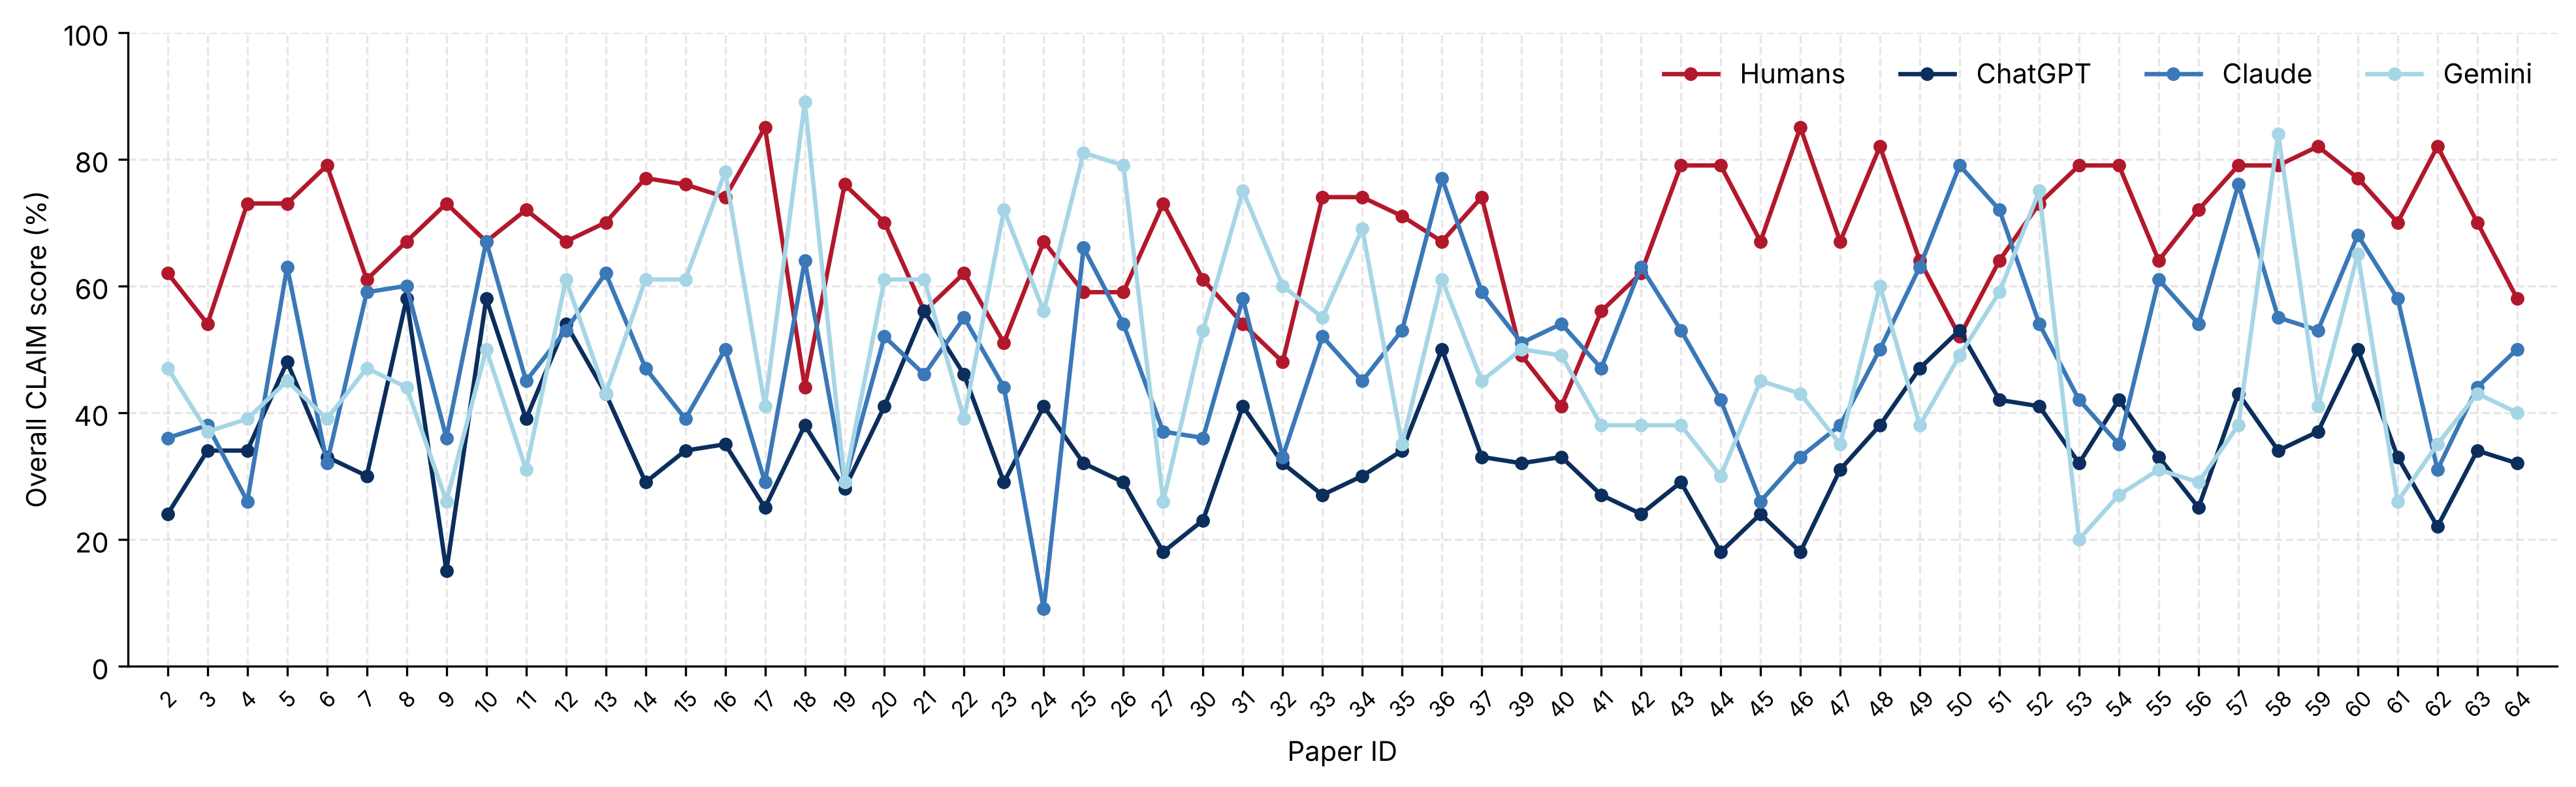
\includegraphics[width=0.8\linewidth]{images/35ScoresResults2.png}
    \caption{Comparison of CLAIM overall scores assigned by humans and LLMs.}
    \label{fig:Scorespaper}
\end{figure}
\vspace{-0.5cm}
\noindent
The boxplots in Figure \ref{fig:scoreDistribution} showed  the majority of human evaluations were between 62-77\%. The three LLMs gave lower and more dispersed scores for the majority of the observations: ChatGPT had a range of 28–41\%, Gemini of 38–61\% and Claude of 38–59\%. 

As it can be seen in bar plots in Figure \ref{fig:scoreDomain}, human evaluators gave the highest mean compliance to Model description (87.00\%) and the lowest to Dataset description (61.70\%). LLMs had their lowest-scored domain in Model description, for ChatGPT (19.17\%) and Claude (29.63\%); Gemini was the exception (57.42\%). In contrast, Performance became the highest-scored domain for all three LLMs (67.98-77.47\%), exceeding the human score (64.00\%). 
\vspace{-0.5cm}
\begin{figure}[H]
    \centering
    \captionsetup[subfigure]{font=scriptsize}
    \begin{subfigure}{0.38\linewidth}
        \centering
        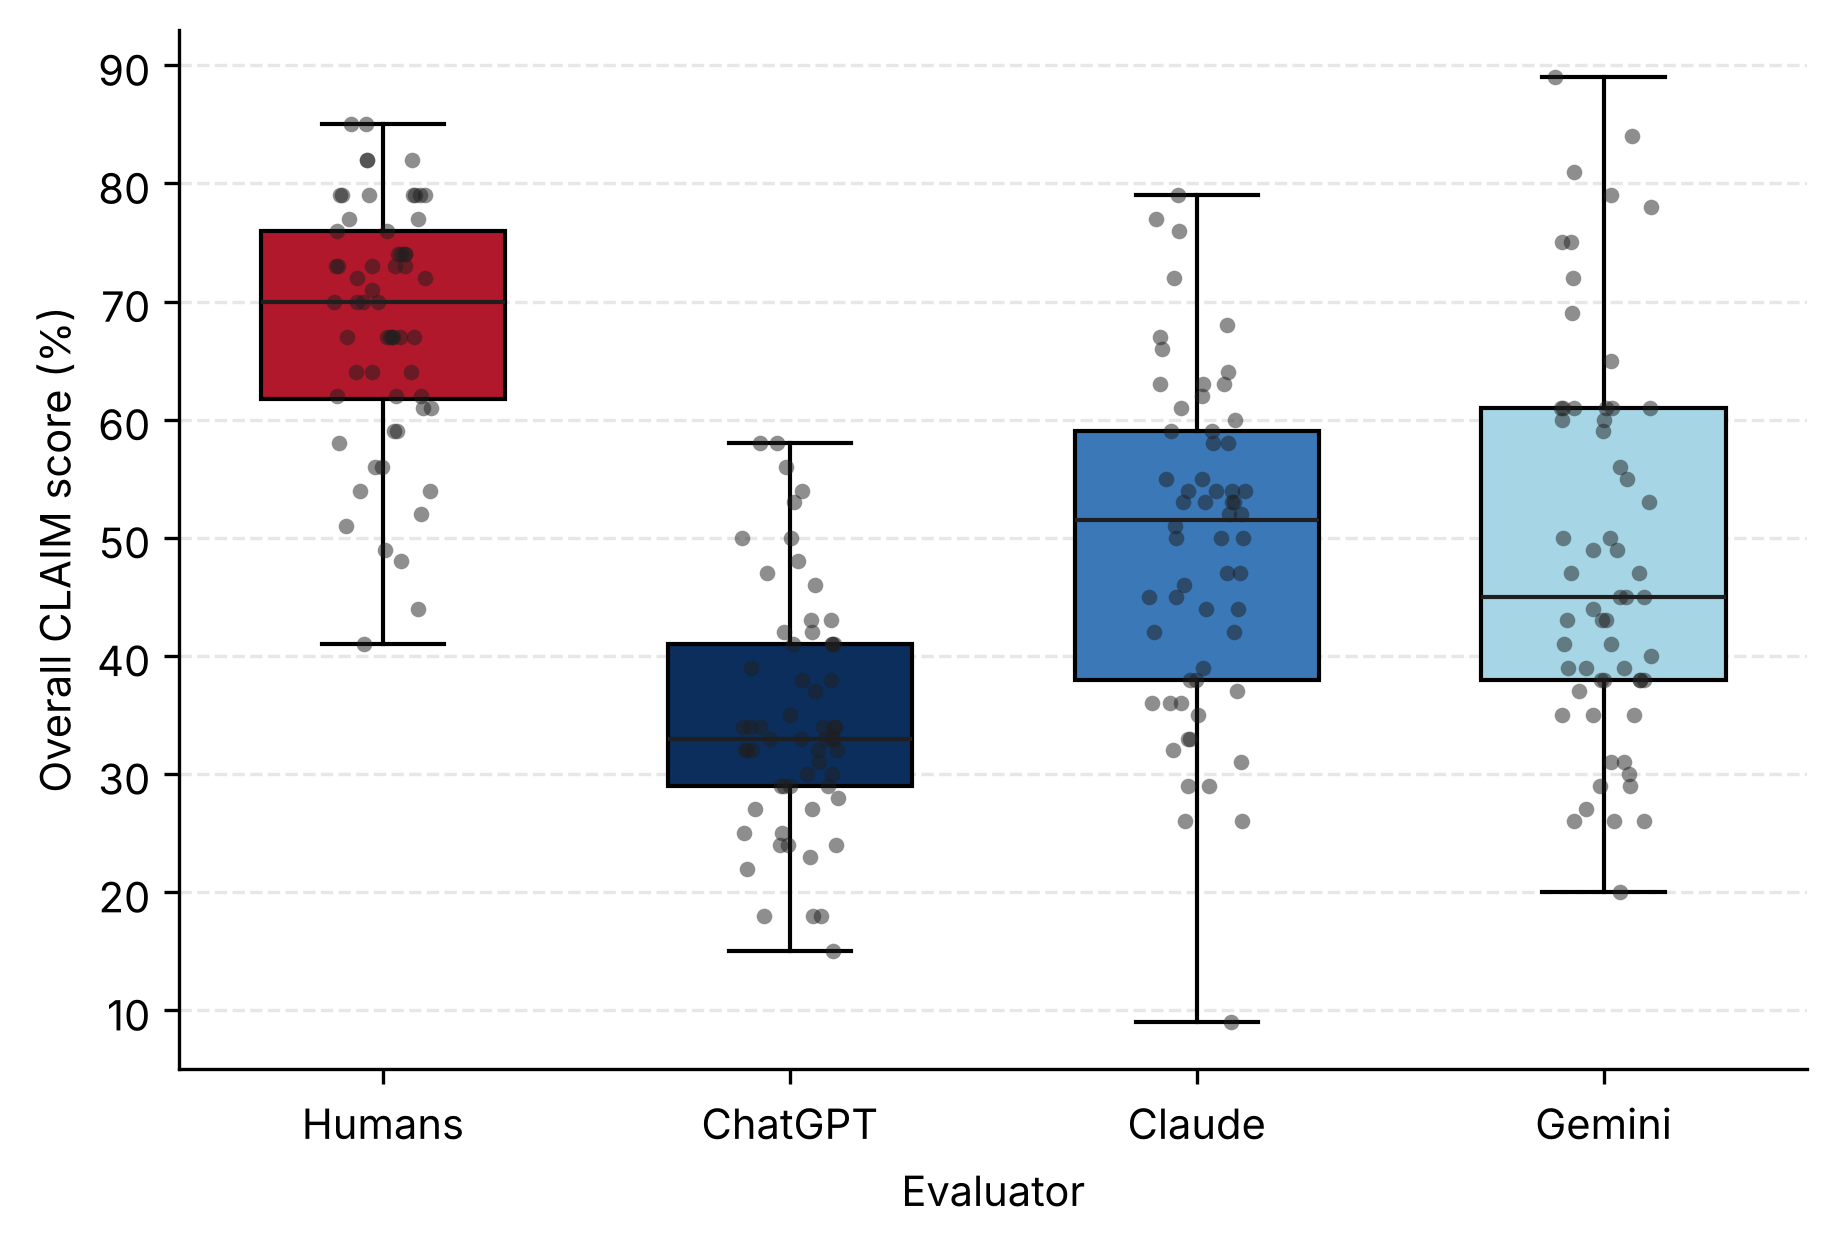
\includegraphics[height=3cm]{images/4ScoresDistribution2.png}
        \caption{}
        \label{fig:scoreDistribution}
    \end{subfigure}
    \hfill
    \begin{subfigure}{0.52\linewidth}
        \centering
        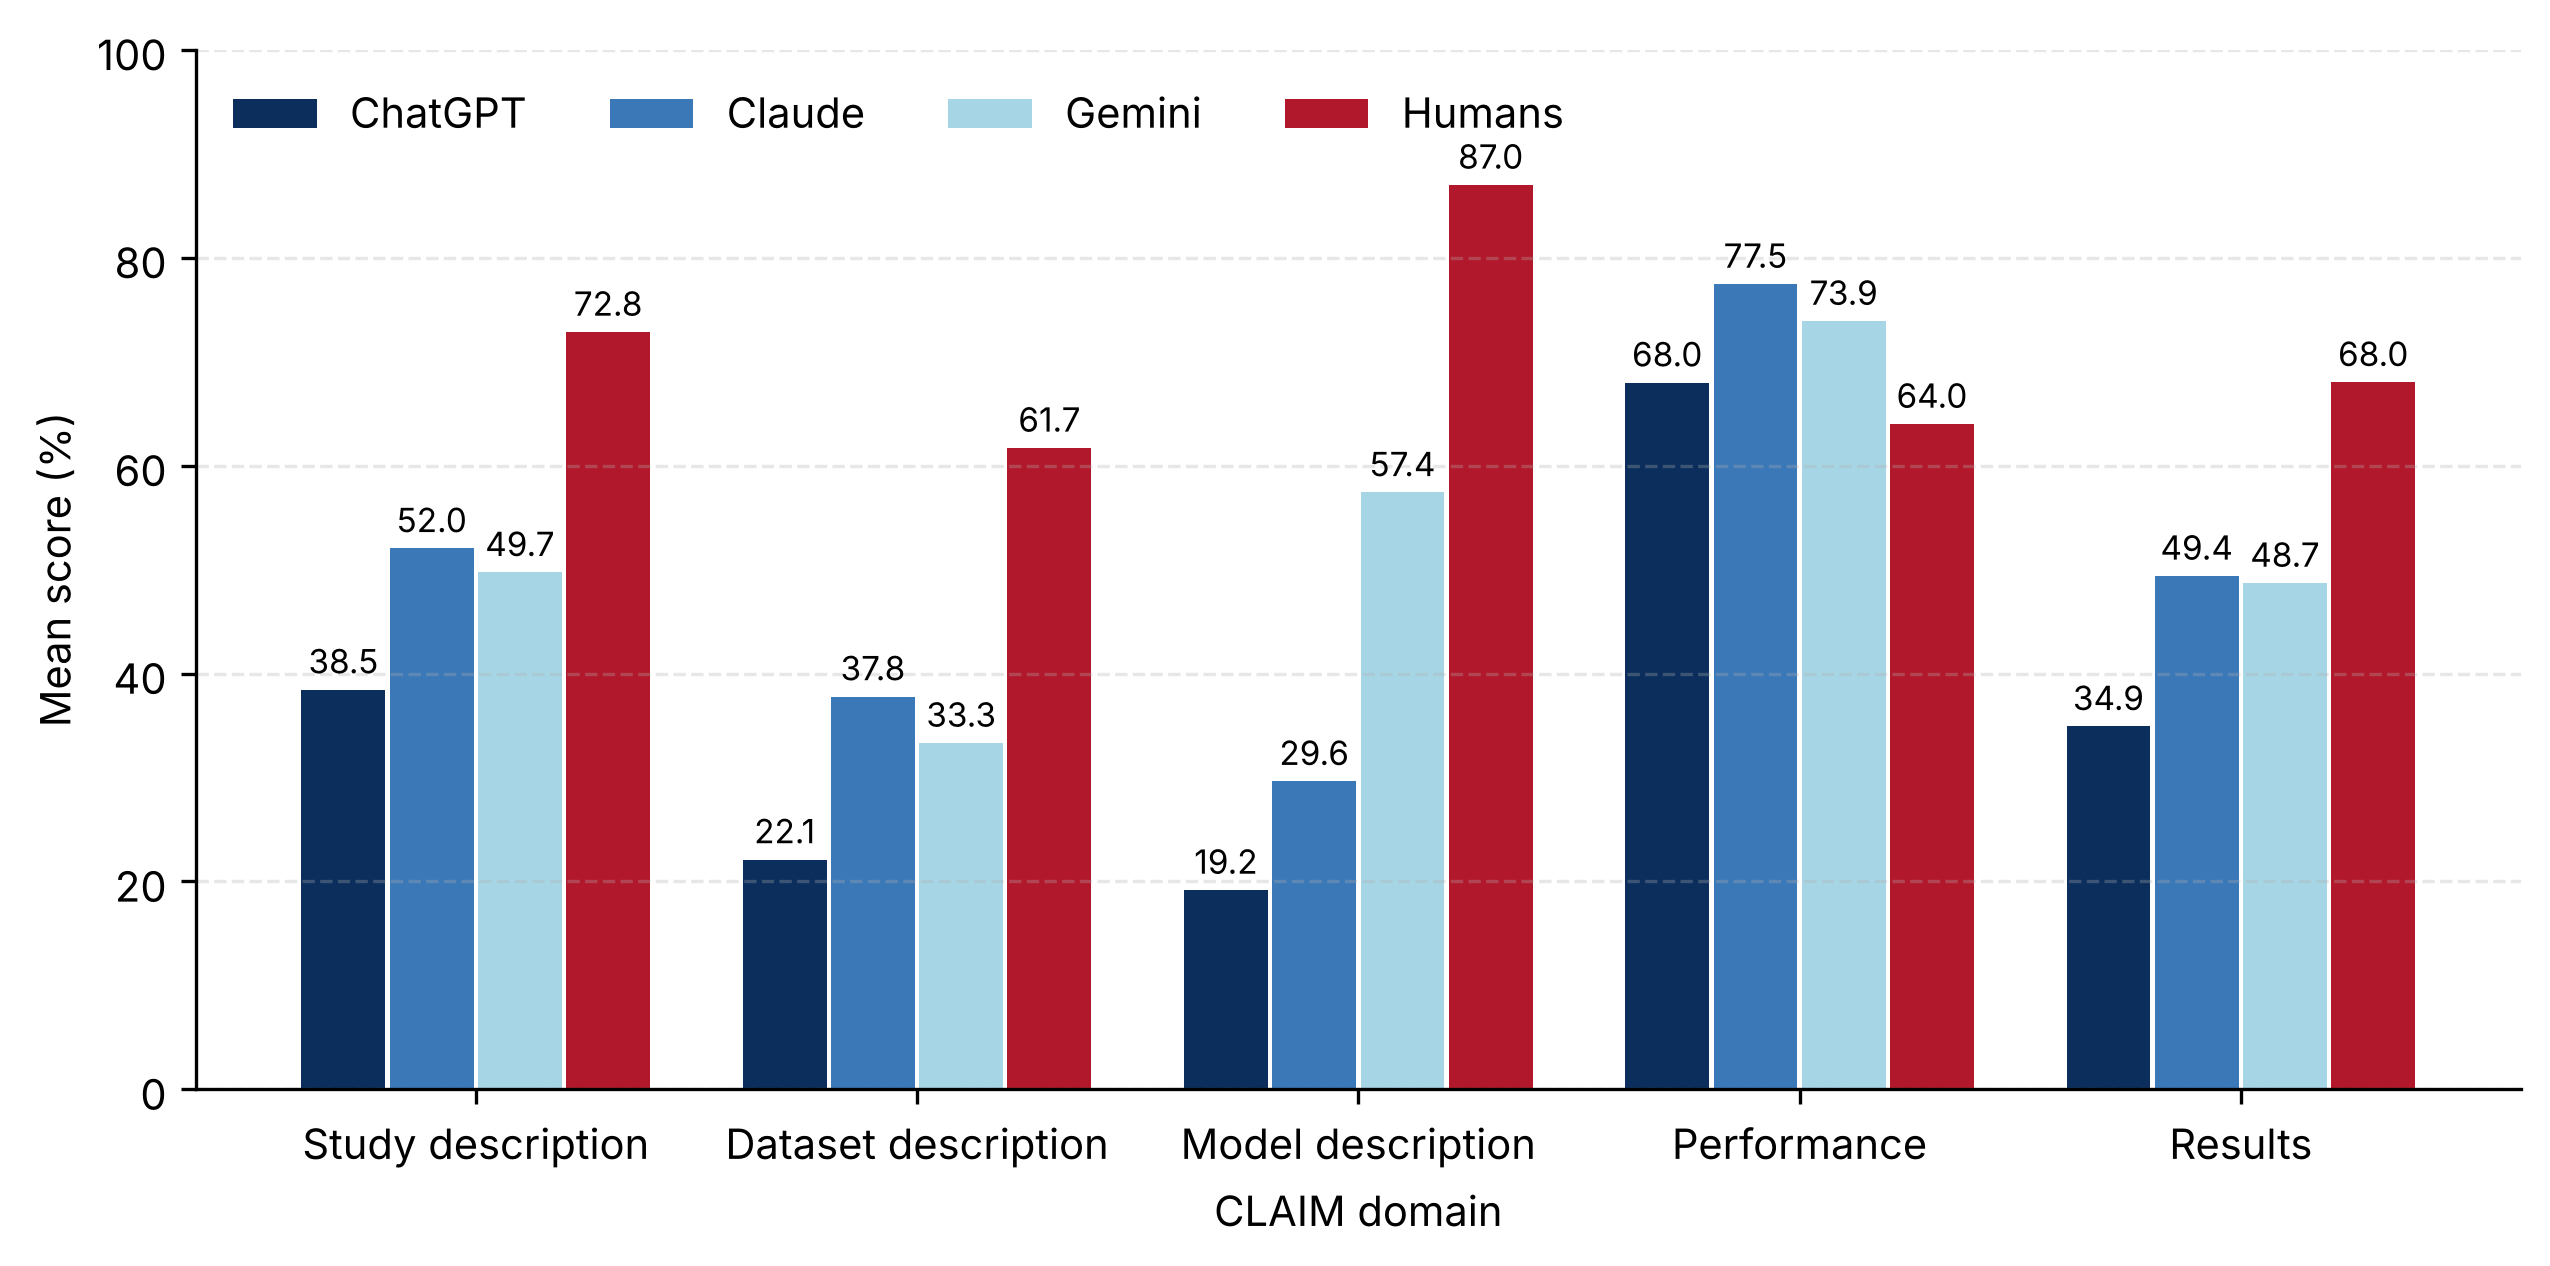
\includegraphics[height=3cm]{images/5ScoresDomain2.png}
        \caption{}
        \label{fig:scoreDomain}
    \end{subfigure}
    \caption{Comparison of CLAIM scores assigned by human and LLM evaluators. (a) Distribution of overall scores. (b) Mean scores across assessment domains.}
    \label{fig:scoreComparison}
\end{figure}
\vspace{-0.5cm}
\noindent
Additionally, evaluation scores were also examined across study metadata variables, ranging from ~10\% to 90\% with unequal sample sizes per category (Appendix \ref{app:scatterplot}). Across all variables, human scores remained consistently clustered at higher values, whereas LLM scores showed wider dispersion and variable overlap. 

\subsection{Agreement and strictness of LLMs compared to human evaluations}
As it can be seen in Table \ref{tab:mae_wilcoxon}, in three of the four CLAIM domains, all LLMs were significantly stricter than human reviewers (ME: $-18.6$ to $-67.8$ pp), with the largest discrepancies in Model description (MAE: 68.5, 61.9, and 42.5 for ChatGPT, Claude, and Gemini, respectively). Claude showed the lowest MAE in Results (21.7), whereas ChatGPT showed the highest (33.13). In Performance, Claude and Gemini were significantly more lenient (ME = 13.5 and 9.9 pp), while ChatGPT showed no significance (ME = 4.0 pp). Overall, 12 of 15 model domain comparisons showed negative bias, and 14 of 15 biases were statistically significant after multiple-comparison correction.
\vspace{-0.5cm}
\begin{table}[H]
\centering
\caption{MAE, ME and Wilcoxon test results comparing LLM and human scores.}
\label{tab:mae_wilcoxon}
\footnotesize
\setlength{\tabcolsep}{6pt}
\renewcommand{\arraystretch}{1.3}
\resizebox{\textwidth}{!}{
\begin{tabular}{llrrrrl}
\hline
\textbf{Target} & \textbf{Model} & \textbf{MAE} & \textbf{ME} &
\textbf{Wilcoxon p} & \textbf{Adjusted p} & \textbf{Direction} \\
\hline
Study description & ChatGPT & 34.600 & -34.400 & $3.58 \times 10^{-11}$ & $4.66 \times 10^{-10}$ & Stricter \\
Study description & Claude  & 25.383 & -20.817 & $1.39 \times 10^{-7}$  & $9.75 \times 10^{-7}$ & Stricter \\
Study description & Gemini  & 29.083 & -23.117 & $1.43 \times 10^{-7}$  & $9.75 \times 10^{-7}$ & Stricter \\
\hline
Dataset description & ChatGPT & 39.700 & -39.600 & $1.79 \times 10^{-11}$ & $2.68 \times 10^{-10}$ & Stricter \\
Dataset description & Claude  & 26.983 & -23.917 & $4.89 \times 10^{-9}$  & $4.89 \times 10^{-8}$ & Stricter \\
Dataset description & Gemini  & 35.150 & -28.383 & $5.71 \times 10^{-8}$  & $4.57 \times 10^{-7}$ & Stricter \\
\hline
Model description & ChatGPT & 68.500 & -67.833 & $6.44 \times 10^{-11}$ & $7.73 \times 10^{-10}$ & Stricter \\
Model description & Claude  & 61.900 & -57.367 & $5.26 \times 10^{-10}$ & $5.79 \times 10^{-9}$ & Stricter \\
Model description & Gemini  & 42.483 & -29.583 & $1.38 \times 10^{-5}$  & $5.53 \times 10^{-5}$ & Stricter \\
\hline
Performance & ChatGPT & 20.517 & 3.983 & $2.18 \times 10^{-1}$ & $2.18 \times 10^{-1}$ & More lenient \\
Performance & Claude  & 25.300 & 13.467 & $8.11 \times 10^{-4}$ & $2.43 \times 10^{-3}$ & More lenient \\
Performance & Gemini  & 22.200 & 9.900 & $4.84 \times 10^{-3}$ & $9.69 \times 10^{-3}$ & More lenient \\
\hline
Results & ChatGPT & 33.133 & -33.100 & $2.50 \times 10^{-11}$ & $3.50 \times 10^{-10}$ & Stricter \\
Results & Claude  & 21.700 & -18.633 & $2.64 \times 10^{-8}$  & $2.37 \times 10^{-7}$ & Stricter \\
Results & Gemini  & 24.850 & -19.317 & $2.18 \times 10^{-7}$  & $1.09 \times 10^{-6}$ & Stricter \\
\hline
\end{tabular}
}
\end{table}
\vspace{-0.5cm}

\subsection{Model differences}
Friedman test results from Table \ref{tab:freidman} revealed significant differences between LLMs in three of the four domains and in the overall score (all adjusted p < 0.001), with no significant difference in Performance (adjusted p = 0.052). Pairwise comparisons showed that Claude was significantly closer to human assessments than ChatGPT in Study description, Dataset description, and Results; and closer than Gemini in Dataset description. Gemini was closer to humans than both ChatGPT and Claude in Model description and closer than ChatGPT in Results. 
\vspace{-0.5cm}
\begin{table}[H]
\centering
\caption{Friedman test results comparing LLM scores across CLAIM domains.}
\label{tab:freidman}
\begin{tabular}{lccc}
\hline
\textbf{Domain} & \textbf{Friedman $\chi^2$} & \textbf{Adjusted p} & \textbf{Significant pairwise comparisons} \\
\hline
Study description   & 16.58 & $<0.001$ & ChatGPT vs \textbf{Claude} \\
Dataset description & 25.93 & $<0.001$ & ChatGPT vs \textbf{Claude}, \textbf{Claude} vs Gemini\\
Model description   & 20.79 & $<0.001$ & ChatGPT vs \textbf{Gemini}, Claude vs \textbf{Gemini} \\
Performance         & 5.93  & 0.052    & None  \\
Results             & 32.67 & $<0.001$ & ChatGPT vs \textbf{Claude}, ChatGPT vs \textbf{Gemini}\\
\hline
\end{tabular}
\begin{minipage}{\textwidth}
\vspace{2mm}
\footnotesize{\textit{Note.} The model in bold is the one more similar to human assessments in each pairwise comparison.}
\end{minipage}
\end{table}
\subsection{Rank correlation}
Spearman correlations of Figure \ref{fig:Spearman} showed no significant association between any LLM and the human evaluations in any CLAIM domain ($(\rho)$ between -0.29 and 0.02), indicating that the LLMs did not rank papers in the same order as human reviewers. The weakest correlations were observed for Dataset description (Gemini, $(\rho)$ = -0.29) and Results (Gemini, $(\rho)$ = -0.27). 

In contrast, agreement among LLMs was higher, with 6 of the 15 pairwise correlations being significant after multiple-testing adjustment. It was strongest between ChatGPT and Claude in Study description ($(\rho)$ = 0.65), Dataset description ($(\rho)$ = 0.62) and Results ($(\rho)$ = 0.54), while Model description showed the lowest agreement ($(\rho)$ = 0.13-0.33, none significant). 
\vspace{-0.5cm}
\begin{figure}[H]
    \centering
    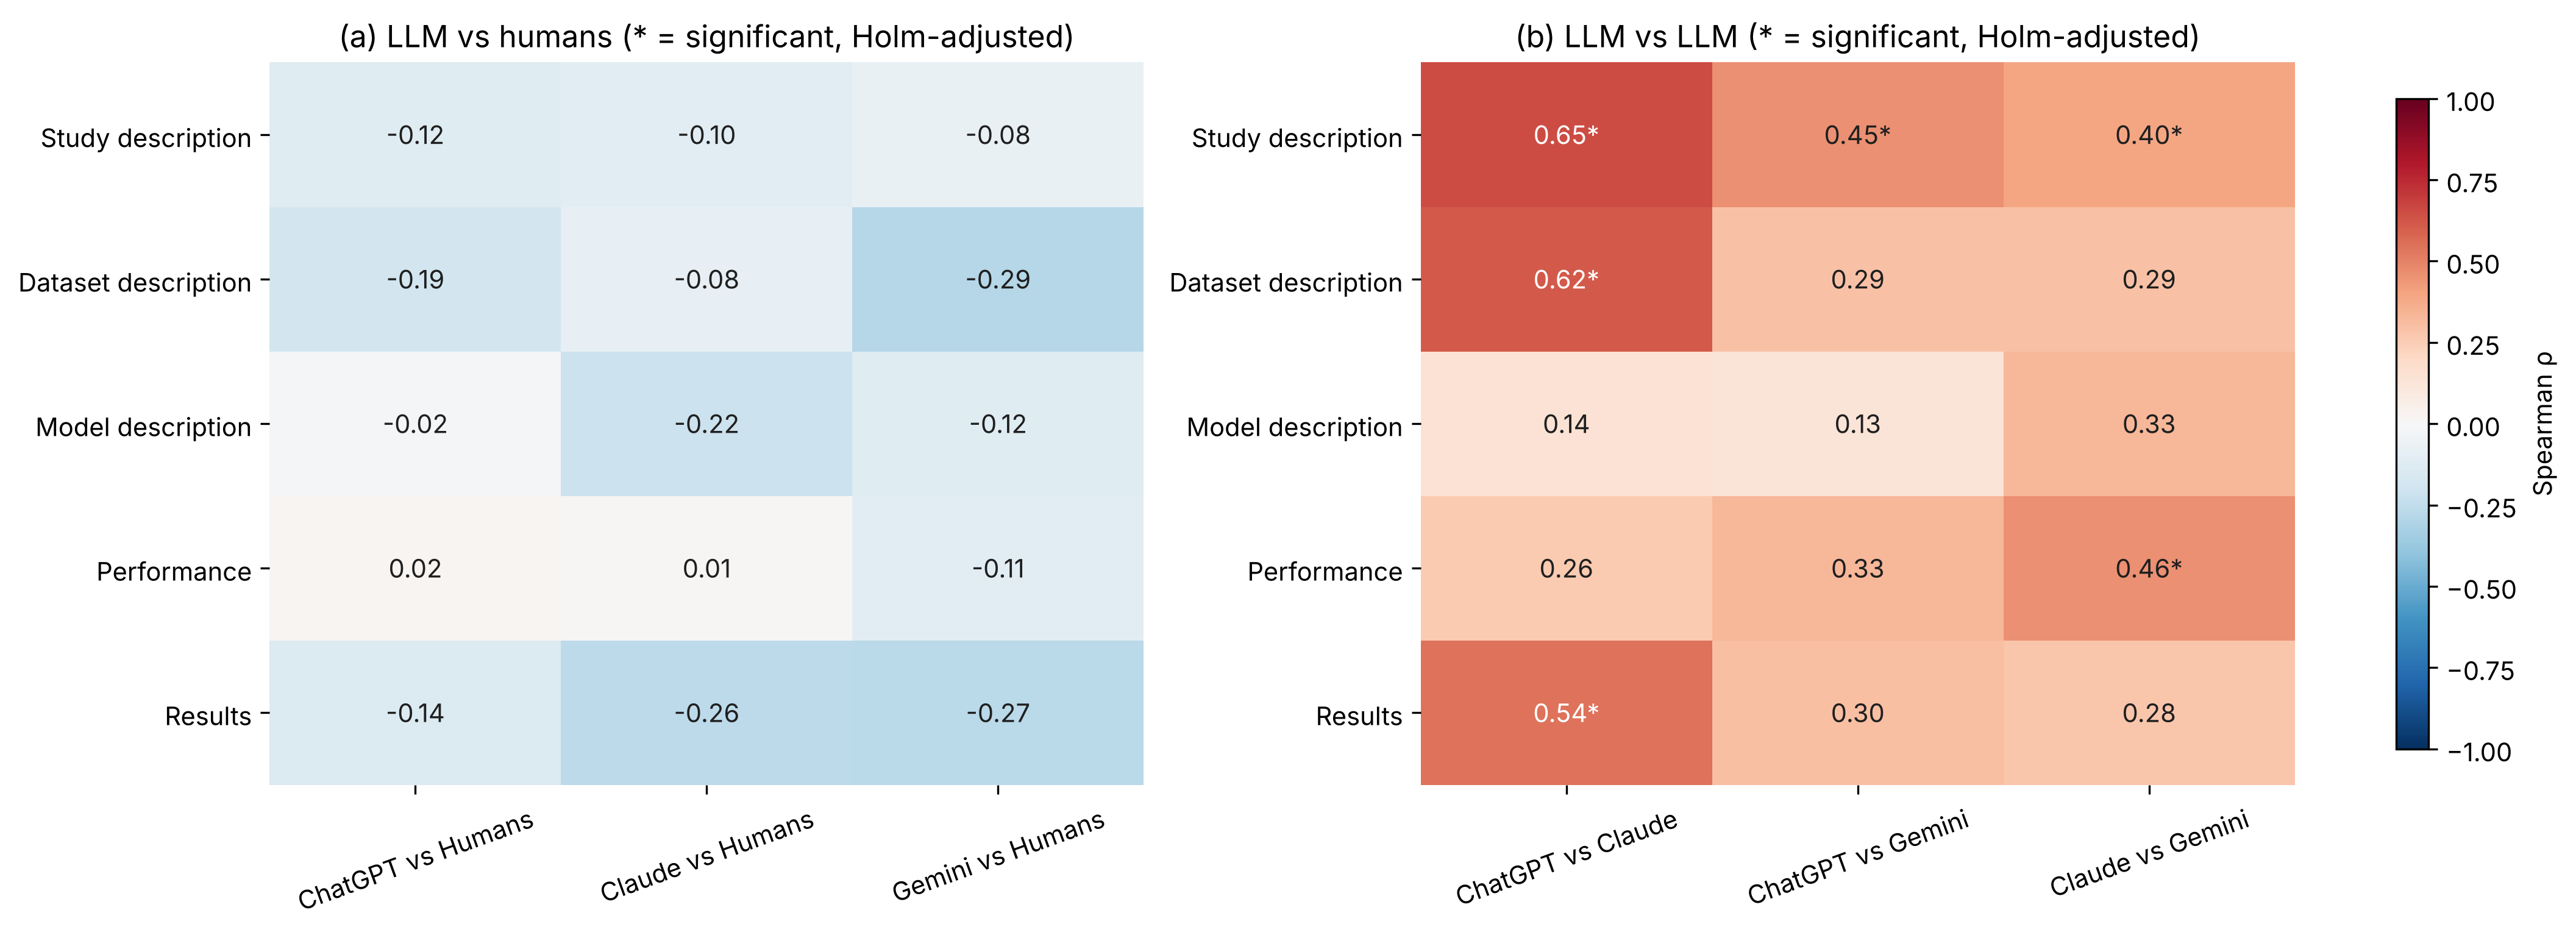
\includegraphics[width=0.9\linewidth]{images/2Spearmanrho.png}
    \caption{Spearman correlation coefficients across CLAIM domains for (a) LLM and human assessments and (b) pairs of LLMs.}
    \label{fig:Spearman}
\end{figure}
\vspace{-0.5cm}


%\begin{figure}[H]
%    \centering
%    \includegraphics[width=1\linewidth]{images/6Metadataresults2.png}
%    \caption{Relationship between overall CLAIM evaluation scores and selected study metadata (performance evaluation, public code availability and link type), stratified by evaluator. Each point represents an individual assessment, with colours distinguishing evaluators.}
%    \label{fig:Metadata}
%\end{figure}


\section{Discussion}
The results reveal important limitations in the use of LLMs to assess CLAIM compliance. Agreement with human assessors was low, with an overall MAE of 21.7-33.1 pp. The models were systematically stricter than humans in all domains except Performance, possibly because they were instructed to rely only on explicitly reported information, whereas humans may accept implicit or partial information. In contrast, Performance showed the opposite pattern, potentially because LLMs considered an item fulfilled once a metric was reported, while humans also evaluated its adequacy. These differences could not be verified at item level.

Furthermore, correlations between LLM and human scores were low ($\rho$ = -0.29 to 0.02), whereas agreement between models was higher (up to $\rho$ = 0.65). This suggests that LLMs may interpret CLAIM differently from human reviewers and rank papers differently, meaning that correcting their systematic bias alone would not ensure agreement. These findings should also be considered in light of the limited range of human scores and the use of a single human assessment team.

Regarding model differences, ChatGPT showed the lowest agreement with human assessors, with the highest MAE in four of five scores. Claude and Gemini showed comparable overall agreement, each performing better in a different domain. This model dependence is consistent with \cite{pluimer-2026}. Unlike \cite{zancanaro-2026}, we did not find LLM scores to be comparable to human assessments, possibly because reproducing item-by-item judgements is more demanding than generating a structured review.




\section{Conclusions}

In conclusion, none of the three LLMs reliably reproduced human CLAIM assessments across the 60 evaluated papers and no single model consistently achieved the highest agreement with human assessments. ChatGPT generally showed the largest discrepancies, whereas Claude and Gemini performed better in different domains. Correlations with human scores were low and non-significant, indicating that the models also rank papers differently from humans.

Within the scope of this study, general-purpose LLMs are not yet reliable substitutes for human CLAIM assessment under the conditions tested, and their use in peer review should remain supervised. Item-level analyses are needed to identify where their judgments can be trusted.

\subsection{Limitations and improvements}
This study has several limitations. First, the lack of item-level human assessments prevented us from identifying which specific CLAIM items were responsible for disagreements. Moreover, human scores may be subject to some degree of subjectivity, meaning that our results reflect disagreement rather than absolute accuracy. Second, the sample was limited to the first 60 available papers from a single imaging field and used CLAIM 2020, limiting the generalization of the findings. Finally, only one prompt and one run per paper were tested using the free versions of the models, preventing assessment of prompt sensitivity and run-to-run variability.

Future work should focus on item-level comparisons, include human-human agreement as a reference, and evaluate multiple prompts and repeated runs. Larger datasets, additional imaging domains, CLAIM 2024 and models with extended reasoning should also be explored. Finally, simple baselines and calibration or fine-tuning strategies could help determine whether LLM reliability can be improved and establish their added value in CLAIM assessment.


\pages 
%
% ---- Bibliography ----
%
% BibTeX users should specify bibliography style 'splncs04'.
% References will then be sorted and formatted in the correct style.
%
% \bibliographystyle{splncs04}
% \bibliography{mybibliography}
%

\newpage
\bibliographystyle{splncs04}
\bibliography{references}

\newpage
\appendix
\section{Items and domains}
\label{app:table}

\begin{longtable}{|p{2cm}|c|p{7.2cm}|p{2.8cm}|}
\hline
\textbf{Section} & \textbf{No.} & \textbf{Criteria} & \textbf{Domain} \\
\hline
\endfirsthead
\hline
\textbf{Section} & \textbf{No.} & \textbf{Criteria} & \textbf{Domain} \\
\hline
\endhead
\hline
\endfoot
\footnotesize
\multirow{1}{=}{\textbf{Title}}
 & 1 & Identification as a study of AI methodology, specifying the category of technology used (e.g., deep learning) & Study description \\
\hline
\multirow{1}{=}{\textbf{Abstract}}
 & 2 & Structured summary of study design, methods, results, and conclusions & Study description \\
\hline
\multirow{2}{=}{\textbf{Introduction}}
 & 3 & Scientific and clinical background, including the intended use and clinical role of the AI approach & Study description \\
\cline{2-4}
 & 4 & Study objectives and hypotheses & Study description \\
\hline
\multirow{2}{=}{\textbf{Study design}}
 & 5 & Prospective or retrospective study & Study description \\
\cline{2-4}
 & 6 & Study goal, such as model creation, exploratory study, feasibility study, non-inferiority trial & Study description \\
\hline
\multirow{7}{=}{\textbf{Data sources}}
 & 7 & Data sources & Dataset description \\
\cline{2-4}
 & 8 & Eligibility criteria: how, where, and when potentially eligible participants or studies were identified (e.g., symptoms, results from previous tests, inclusion in registry, patient-care setting, location, dates) & Dataset description \\
\cline{2-4}
 & 9 & Data pre-processing steps & Dataset description \\
\cline{2-4}
 & 10 & Selection of data subsets, if applicable & Dataset description \\
\cline{2-4}
 & 11 & Definitions of data elements, with references to Common Data Elements & Dataset description \\
\cline{2-4}
 & 12 & De-identification methods & Dataset description \\
\cline{2-4}
 & 13 & How missing data were handled & Dataset description \\
\hline
\multirow{5}{=}{\textbf{Ground truth reference standard}}
 & 14 & Definition of ground truth reference standard, in sufficient detail to allow replication & Dataset description \\
\cline{2-4}
 & 15 & Rationale for choosing the reference standard (if alternatives exist) & Dataset description \\
\cline{2-4}
 & 16 & Source of ground-truth annotations; qualifications and preparation of annotators & Dataset description \\
\cline{2-4}
 & 17 & Annotation tools & Dataset description \\
\cline{2-4}
 & 18 & Measurement of inter- and intrarater variability; methods to mitigate variability and/or resolve discrepancies & Dataset description \\
\hline
\multirow{3}{=}{\textbf{Data partitions}}
 & 19 & Intended sample size and how it was determined & Dataset description \\
\cline{2-4}
 & 20 & How data were assigned to partitions; specify proportions & Dataset description \\
\cline{2-4}
 & 21 & Level at which partitions are disjoint (e.g., image, study, patient, institution) & Dataset description \\
\hline
\multirow{3}{=}{\textbf{Model}}
 & 22 & Detailed description of model, including inputs, outputs, all intermediate layers and connections & Model description \\
\cline{2-4}
 & 23 & Software libraries, frameworks, and packages & Model description \\
\cline{2-4}
 & 24 & Initialization of model parameters (e.g., randomization, transfer learning) & Model description \\
\hline
\multirow{3}{=}{\textbf{Training}}
 & 25 & Details of training approach, including data augmentation, hyperparameters, number of models trained & Model description \\
\cline{2-4}
 & 26 & Method of selecting the final model & Model description \\
\cline{2-4}
 & 27 & Ensembling techniques, if applicable & Model description \\
\hline
\multirow{5}{=}{\textbf{Evaluation}}
 & 28 & Metrics of model performance & Model performance \\
\cline{2-4}
 & 29 & Statistical measures of significance and uncertainty (e.g., confidence intervals) & Model performance \\
\cline{2-4}
 & 30 & Robustness or sensitivity analysis & Model performance \\
\cline{2-4}
 & 31 & Methods for explainability or interpretability (e.g., saliency maps), and how they were validated & Model performance \\
\cline{2-4}
 & 32 & Validation or testing on external data & Model performance \\
\hline
\multirow{2}{=}{\textbf{Data}}
 & 33 & Flow of participants or cases, using a diagram to indicate inclusion and exclusion & Dataset description \\
\cline{2-4}
 & 34 & Demographic and clinical characteristics of cases in each partition & Dataset description \\
\hline
\multirow{3}{=}{\textbf{Model performance}}
 & 35 & Performance metrics for optimal model(s) on all data partitions & Model performance \\
\cline{2-4}
 & 36 & Estimates of diagnostic accuracy and their precision (such as 95\% confidence intervals) & Model performance \\
\cline{2-4}
 & 37 & Failure analysis of incorrectly classified cases & Model performance \\
\hline
\multirow{2}{=}{\textbf{Discussion}}
 & 38 & Study limitations, including potential bias, statistical uncertainty, and generalizability & Model performance \\
\cline{2-4}
 & 39 & Implications for practice, including the intended use and/or clinical role & Model performance \\
\hline
\multirow{3}{=}{\textbf{Other information}}
 & 40 & Registration number and name of registry & Study description \\
\cline{2-4}
 & 41 & Where the full study protocol can be accessed & Study description \\
\cline{2-4}
 & 42 & Sources of funding and other support; role of funders & Study description \\
\end{longtable}

\newpage
\section{Prompt used for LLM CLAIM evaluation}
\label{app:prompt}
“Act as an experienced scientific peer reviewer with expertise in artificial intelligence (AI) and medical imaging research. Your task is to critically assess the attached scientific manuscript using the 2020 version of the Checklist for Artificial Intelligence in Medical Imaging (CLAIM). Your assessment must reflect the judgment and rigor of an independent human reviewer.

Every time a new PDF is provided, perform the complete evaluation from the beginning, applying all 42 items of the CLAIM 2020 checklist and following all the instructions below. Treat each PDF as an independent manuscript. Do not use information, assessments, conclusions, or assumptions from previously evaluated PDFs. Do not compare the current manuscript with previously evaluated manuscripts. The evaluation criteria, interpretation of the response categories, and output format must remain exactly the same for every PDF.

Instructions:

1. Assess all 42 items individually and independently. Do not skip, combine, or reorder any items.

2. For each item, assign exactly one of the following answers:
   - Yes: The manuscript adequately addresses the item. The information provided is sufficiently clear and detailed to satisfy the criterion.
  - No: The manuscript does not address the item, or the information provided is insufficient, incomplete, unclear, or inadequate to satisfy the criterion.
   - Not applicable (N/A): The item is genuinely not applicable to the study because of its design, methodology, or research objectives.

3. Use only information explicitly reported in the manuscript. Do not assume that the authors performed a procedure, analysis, validation, or methodological step unless it is described in the paper. Do not fill reporting gaps using common scientific practices, external knowledge, or assumptions about what the authors probably did.

4. Distinguish between missing information and non-applicability. If an item is relevant to the study but the authors fail to report the required information, assign No rather than N/A. Use N/A only when the criterion genuinely does not apply to the particular study.

5. Consider the entire manuscript, including the abstract, introduction, methods, results, discussion, conclusions, tables, figures, figure captions, supplementary materials, and appendices, if provided. Information may be reported in different sections of the paper.

6. Do not evaluate whether the study's scientific conclusions are correct or whether the AI model performs well. Your task is specifically to assess the completeness and quality of reporting according to the CLAIM checklist.

7. Do not provide explanations, justifications, comments, recommendations, summaries, or additional observations in your response.

Output format: Return exactly 43 lines, one for pdf name and one for each checklist item, in the following format:

\begin{enumerate}
    \item Yes
    \item No
    \item Not applicable
    \setcounter{enumi}{41}
    
    \dots
    
    \item Yes
\end{enumerate}

Use the original item numbers from the checklist. Do not include an introduction, heading, conclusion, additional formatting, or any text outside these 42 lines.\\


\noindent
CLAIM 2020 checklist:

Item 1. Indicate the use of the AI techniques—such as “deep learning” or “random forests”—in the article’s title and/or abstract; use judgment regarding the level of specificity.

Item 2. The abstract should present a structured summary of the study’s design, methods, results, and conclusions; it should be understandable without reading the entire manuscript. Provide an overview of the study population (number of patients or examinations, number of images, age and sex distribution). Indicate if the study is prospective or retrospective, and summarize the statistical analysis that was performed. When presenting the results, be sure to include P values for any comparisons. Indicate whether the software, data, and/or resulting model are available publicly.

Item 3. Address an important clinical, scientific, or operational issue. Describe the study’s rationale, goals, and anticipated impact. Summarize related literature and highlight how the investigation builds upon and differs from that work. Guide readers to understand the context for the study, the underlying science, the assumptions underlying the methodology, and the nuances of the study.

Item 4. Define clearly the clinical or scientific question to be answered; avoid vague statements or descriptions of a process. Limit the chance of post hoc data dredging by specifying the study’s hypothesis a priori. Identify a compelling problem to address. The study’s objectives and hypothesis will guide sample size calculations and whether the hypothesis will be supported or not.

Item 5. Indicate if the study is retrospective or prospective. Evaluate predictive models in a prospective setting, if possible.

Item 6. Define the study’s goal, such as model creation, exploratory study, feasibility study, or non inferiority trial. For classification systems, state the intended use, such as diagnosis, screening, staging, monitoring, surveillance, prediction, or prognosis (2). Indicate the proposed role of the AI algorithm relative to other approaches, such as triage, replacement, or add-on (2). Describe the type of predictive modeling to be performed, the target of predictions, and how it will solve the clinical or scientific question.

Item 7. State the source of data and indicate how well the data match the intended use of the model. Describe the targeted application of the predictive model to allow readers to interpret the implications of reported accuracy estimates. Reference any previous studies that used the same dataset and specify how the current study differs. Adhere to ethical guidelines to assure that the study is conducted appropriately; describe the ethics review and informed consent (19). Provide links to data sources and/or images, if available. Authors are strongly encouraged to deposit data and/or software used for modeling or data analysis in a publicly accessible repository.

Item 8. Define how, where, and when potentially eligible participants or studies were identified. Specify inclusion and exclusion criteria such as location, dates, patient-care setting, symptoms, results from previous tests, or registry inclusion. Indicate whether a consecutive, random, or convenience series was selected. Specify the number of patients, studies, reports, and/or images.

Item 9. Preprocessing converts raw data from various sources into a well-defined, machine-readable format for analysis (20,21). Describe preprocessing steps fully and in sufficient detail so that other investigators could reproduce them. Specify the use of normalization, resampling of image size, change in bit depth, and/or adjustment of window/level settings. State whether or not the data have been rescaled, threshold-limited (“binarized”), and/or standardized. Specify how the following issues were handled: regional format, manual input, inconsistent data, missing data, wrong data types, file manipulations, and missing anonymization. Define any criteria to remove outliers (11). Specify the libraries, software (including manufacturer name and location), and version numbers, and all option and configuration settings employed.

Item 10. In some studies, investigators select subsets of the raw extracted data as a preprocessing step, for instance, selecting a subset of the images, cropping down to a portion of an image, or extracting a portion of a report. If this process is automated, describe the tools and parameters used; if done manually, specify the training of the personnel and the criteria they used. Justify how this manual step would be accommodated in the context of the clinical or scientific problem to be solved.

Item 11. Define the predictor and outcome variables. Map them to common data elements, if applicable, such as those maintained by the radiology community (22–24) or the U.S. National Institutes of Health (25,26).

Item 12. Describe the methods by which data have been de-identified and how protected health information has been removed to meet U.S. (HIPAA), European (GDPR), or other relevant laws. Because facial profiles can allow identification, specify the means by which such information has been removed or made unidentifiable (20).

Item 13. State clearly how missing data were handled, such as replacing them with approximate or predicted values. Describe the biases that the imputed data might introduce.

Item 14. Include detailed, specific definitions of the ground truth annotations, ideally referencing common data elements. Avoid vague descriptions such as “size of liver lesion;” use more precise definitions, such as “greatest linear measurement in millimeters passing entirely through the lesion as measured on axial contrast-enhanced CT images of 2.5-mm thickness.” Provide an atlas of examples to annotators to illustrate subjective grading schemes (eg, mild/moderate/severe), and make that information available for review.

Item 15. Describe the rationale for the choice of the reference standard and the potential errors, biases, and limitations of that reference standard.

Item 16. Specify the number of human annotators and their qualifications. Describe the instructions and training given to annotators; include training materials as a supplement, if possible. Describe whether annotations were done independently and how any discrepancies among annotators were resolved.

Item 17. Specify the software used for manual, semi automated, or automated annotation, including the version number. Describe if and how imaging labels were extracted from free-text imaging reports or electronic health records using natural language processing or recurrent neural networks (20,27,28).

Item 18. Describe the methods to measure inter- and intrarater variability, and any steps taken to reduce or mitigate this variability and/or resolve discrepancies.

Item 19. Describe the sample size and how it was determined. Use traditional power calculation methods, if applicable, to estimate the required sample size to allow for generalizability in a larger population and how many cases are needed to show an effect (29).

Item 20. Specify how the data were assigned into training, validation (“tuning”), and testing partitions; indicate the proportion of data in each partition and justify that selection. Indicate if there are any systematic differences between the data in each partition, and if so, why.

Item 21. Describe the level at which the partitions are disjoint. Sets of medical images generally should be disjoint at the patient level or higher so that images of the same patient do not appear in each partition.

Item 22. Provide a complete and detailed structure of the model, including inputs, outputs, and all intermediate layers, in sufficient detail that another investigator could exactly reconstruct the network. For neural network models, include all details of pooling, normalization, regularization, and activation in the layer descriptions. Model inputs must match the form of the preprocessed data. Model outputs must correspond to the requirements of the stated clinical problem, and for supervised learning should match the form of the ground truth annotations. If a previously published model architecture is employed, cite a reference that meets the preceding standards and fully describe every modification made to the model. In some cases, it may be more convenient to provide the structure of the model in code as supplemental data.

Item 23. Specify the names and version numbers of all software libraries, frameworks, and packages. Avoid detailed description of hardware unless benchmarking computational performance is a focus of the work.

Item 24. Indicate how the parameters of the model were initialized. Describe the distribution from which random values were drawn for randomly initialized parameters. Specify the source of the starting weights if transfer learning is employed to initialize parameters. When there is a combination of random initialization and transfer learning, make it clear which portions of the model were initialized with which strategies.

Item 25. Completely describe all of the training procedures and hyperparameters in sufficient detail that another investigator could exactly duplicate the training process. Typically, to fully document training, a manuscript would: Describe how training data were augmented (eg, for images the types and ranges of transformations). State how convergence of training of each model was monitored and what the criteria for stopping training were. Indicate the values that were used for every hyperparameter, which of these were varied between models, over what range, and using what search strategy. For neural networks, descriptions of hyperparameters should include at least learning rate schedule, optimization algorithm, minibatch size, dropout rates (if any), and regularization parameters (if any). Discuss what objective function was employed, why it was selected, and to what extent it matches the performance required for the clinical or scientific use case. Define criteria used to select the best-performing model. If some model parameters are frozen or restricted from modification, as is often the case in transfer learning, clearly indicate which parameters are involved, the method by which they are restricted, and the portion of the training for which the restriction applies. It may be more concise to describe these details in code in the form of a succinct training script, particularly for neural network models when using a standard framework.

Item 26. Describe the method and performance parameters used to select the best-performing model among all the models trained for evaluation against the held-out test set. If more than one model is selected, justify why this is appropriate.

Item 27. If the final algorithm involves an ensemble of models, describe each model comprising the ensemble in complete detail in accordance with the preceding recommendations. Indicate how the outputs of the component models are weighted and/or combined.

Item 28. Describe the metric(s) used to measure the model’s performance and indicate how they address the performance characteristics most important to the clinical or scientific problem. Compare the presented model to previously published models.

Item 29. Indicate the uncertainty of the performance metrics’ values, such as with standard deviation and/or confidence intervals. Compute appropriate tests of statistical significance to compare metrics. Specify the statistical software.

Item 30. Analyze the robustness or sensitivity of the model to various assumptions or initial conditions.

Item 31. If applied, describe the methods that allow one to explain or interpret the model’s results and provide the parameters used to generate them (14). Describe how any such methods were validated in the current study.

Item 32. Describe the data used to evaluate performance of the completed algorithm. When these data are not drawn from a different data source than the training data, note and justify this limitation. If there are differences in structure of annotations or data between the training set and evaluation set, explain the differences, and describe and justify the approach taken to accommodate the differences.

Item 33. Specify the criteria to include and exclude patients or examinations or pieces of information and document the numbers of cases that met each criterion. We strongly recommend including a flowchart/diagram in your results to show initial patient population and those excluded for any reason. Describe the summary of the technical characteristics of the dataset. For example, for images: modality vendors/models, acquisition parameters, reformat parameters; for reports: practice setting, number and training of report authors, extent of structured reporting.

Item 34. Demographic and clinical characteristics of cases in each partition should be specified. State the performance metrics on all data partitions.

Item 35. Report the final model’s performance on the test partition. Benchmark the performance of the AI model against current standards, such as histopathologic identification of disease or a panel of medical experts with an explicit method to resolve disagreements.

Item 36. For classification tasks, include estimates of diagnostic accuracy and their precision, such as 95\% confidence intervals (2). Apply appropriate methodology such as receiver operating characteristic analysis and/or calibration curves. When the direct calculation of confidence intervals is not possible, report nonparametric estimates from bootstrap samples (11). State which variables were shown to be predictive of the response variable. Identify the subpopulation(s) for which the prediction model worked most and least effectively (11).

Item 37. Provide information to help understand incorrect results. If the task entails classification into two or more categories, provide a confusion matrix that shows tallies for predicted versus actual categories. Consider presenting examples of incorrectly classified cases to help readers better understand the strengths and limitations of the algorithm.

Item 38. Summarize the results succinctly and place them into context; explain how the current work advances our knowledge and the state of the art. Identify the study’s limitations, including those involving the study’s methods, materials, biases, statistical uncertainty, unexpected results, and generalizability.

Item 39. Describe the implications for practice, including the intended use and possible clinical role of the AI model. Describe the key impact the work may have on the field. Envision the next steps that one might take to build upon the results. Discuss any issues that would impede successful translation of the model into practice.

Item 40. Comply with the clinical trial registration statement from the International Committee of Medical Journal Editors (ICMJE). ICMJE recommends that all medical journal editors require registration of clinical trials in a public trials registry at or before the time of first patient enrollment as a condition of consideration for publication (30). Registration of the study protocol in a clinical trial registry, such as ClinicalTrials.gov or WHO Primary Registries, helps avoid overlapping or redundant studies and allows interested parties to contact the study coordinators (5).

Item 41. State where readers can access the full study protocol if it exceeds the journal’s word limit; this information can help readers evaluate the validity of the study and can help researchers who want to replicate the study (5). Describe the algorithms and software in sufficient detail to allow replication of the study. Authors should deposit all computer code used for modeling and/or data analysis into a publicly accessible repository.

Item 42. Specify the sources of funding and other support and the exact role of the funders in performing the study. Indicate whether the authors had independence in each phase of the study”
\newpage

\section{CLAIM evaluation scores by study metadata}
\label{app:scatterplot}
\vspace{-0.5cm}
\begin{figure}[H]
    \centering
    \includegraphics[width=1\linewidth]{images/figC1_scores_by_metadata.png}
    \caption{Relationship between overall CLAIM evaluation scores and selected study metadata, stratified by evaluator.}
    \label{fig:Metadata}
\end{figure}

\end{document}
